\chapter{bottom\_bc}

\section{Purpose}

This test case is used to validate the boundary conditions on the bed fo
\telemac{3D} simulations.

\section{Description of the problem}

In this test case, two simulations are run.
In \telfile{t3d\_bottom\_inlet.cas}, a flow rate is imposed using the boundary
conditions on the bed, whereas in \telfile{t3d\_bottom\_source.cas},
a source discharge is imposed on a node on the bed as a source term.

\subsection{Initial and Boundary Conditions}

A discharge $Q$ of 10,000~m$^3$/s is imposed inside a circle with diameter $D$
of 100~m placed at the centre of the bed.\\
All vertical boundaries are defined as walls, see Figure\ref{fig:GeomPlan}.\\
Nikuradse law with friction coefficient equal to 0.01~m is imposed on the bottom.

The depth is constant, and initially set to 500~m.

\subsection{Geometry and Mesh}

The configuration of this test case is simple, it is a square box of sides
4,000~m.
The geometry of the test case is shown in Figure \ref{fig:GeomPlan}.

\begin{figure}[t!]
\begin{center}
	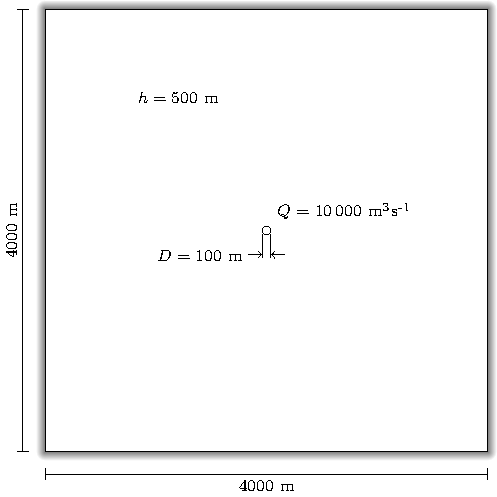
\includegraphics[]{GeomPlan.pdf}
\end{center}
\caption{Geometrical parameters of the test case.}
\label{fig:GeomPlan}
\end{figure}

Furthermore, two different meshes are used, a fine mesh made of 8,336 elements
and 4,233 nodes (Figure \ref{fig:bottom_bc:MeshHinlet}) and a coarse mesh
made of 2,580 elements and 1,355 nodes (Figure \ref{fig:bottom_bc:MeshHsource}).
The finer mesh is more refined around the discus where the discharge is
prescribed.

\begin{figure}[H]
 \centering
 \includegraphicsmaybe{[width=\textwidth]}{../img/Mesh_inlet.png}
  \caption{Horizontal mesh (finer for inlet).}\label{fig:bottom_bc:MeshHinlet}
\end{figure}

\begin{figure}[H]
 \centering
 \includegraphicsmaybe{[width=\textwidth]}{../img/Mesh_source.png}
  \caption{Horizontal mesh (coarser for source).}\label{fig:bottom_bc:MeshHsource}
\end{figure}

Since source terms are imposed on a node, the coarse mesh is used to impose the
inflow on a single node, and it is be used for \telfile{t3d\_bottom\_source.cas}.
Since applying a flow rate can be done on several nodes on the bed,
the finer mesh is compared to the coarse mesh for \telfile{t3d\_bottom\_inlet.cas}
simulation results.
The coarseness of the mesh is also present for the distribution of the planes
in the simulation.
The fine mesh has a smaller plane spacing near the bed and the free surface,
whereas the coarse mesh has the same number of planes, but these are
distributed evenly on the bottom half of the domain and the plane spacing
decreases towards the free-surface.
Both 3D meshes are made of 21 planes (see Figures \ref{fig:bottom_bc:MeshVinlet} and \ref{fig:bottom_bc:MeshVsource}).

\begin{figure}[H]
 \centering
 \includegraphicsmaybe{[width=\textwidth]}{../img/MeshV_inlet.png}
  \caption{Vertical mesh (finer for inlet).}\label{fig:bottom_bc:MeshVinlet}
\end{figure}

\begin{figure}[H]
 \centering
 \includegraphicsmaybe{[width=\textwidth]}{../img/MeshV_source.png}
  \caption{Vertical mesh (coarser for source).}\label{fig:bottom_bc:MeshVsource}
\end{figure}

\subsection{Numerical parameters}

The key numerical parameters for \telfile{t3d\_bottom\_inlet.cas} are:

\begin{itemize}
\item \telkey{OPEN BOUNDARY CONDITIONS ON THE BED = YES}
\item \telkey{PRESCRIBED FLOWRATES ON THE BED = 10000.}
\item \telkey{NON-HYDROSTATIC VERSION = YES}
\end{itemize}

The key numerical parameters for \telfile{t3d\_bottom\_source.cas} are:

\begin{itemize}
\item \telkey{ABSCISSAE OF SOURCES = 2000.0}
\item \telkey{ORDINATES OF SOURCES = 2000.0}
\item \telkey{ELEVATIONS OF SOURCES = -500.0}
\item \telkey{WATER DISCHARGE OF SOURCES = 10000.}
\item \telkey{NON-HYDROSTATIC VERSION = YES}
\end{itemize}

For both steering files, the N-type MURD scheme (scheme 4) is used to solve the
advection of velocities.

The time step is 1~s for the ijnection on the bed and 5~s for the source
discharge, both for a simulated period of 1,800~s.

\section{Results}

%At the moment, no post processing is done, however it would be good to have a
%comparison of the water depth profiles at $y=2000$ m and the vertical velocity
%profiles at $x=2000$ m and $y=2000$ m. Contour plots of the vertical velocities
%at $y=2000$ m would also be useful.

Figure \ref{fig:bottom_bc:waterdepth} shows the water depth profiles along
plane $y$ = 2,000~m for inlet (top) and source (bottom) cases
at different time steps of the simulations.
A clear deformation of the free surface can be seen for the inlet case
more important than for the source case.

\begin{figure}[H]
\centering
\begin{minipage}[t]{1.1\textwidth}
 \centering
\includegraphicsmaybe{[width=\textwidth]}{../img/water_depth_inlet.png}
\end{minipage}
%
\begin{minipage}[t]{\textwidth}
 \centering
\includegraphicsmaybe{[width=\textwidth]}{../img/water_depth_source.png}
\end{minipage}
%
 \caption{Water depth evolution (top for inlet, bottom for source).}
 \label{fig:bottom_bc:waterdepth}
\end{figure}

Figure \ref{fig:bottom_bc:veloH} shows the horizontal velocity
at the free surface for inlet (top) and source (bottom) cases.
A circular symmetry can be seen for the inlet (top) case not
as well reproduced for the source (bottom) case.

\begin{figure}[H]
\centering
\begin{minipage}[t]{.9\textwidth}
 \centering
\includegraphicsmaybe{[width=\textwidth]}{../img/veloH_inlet.png}
\end{minipage}
%
\begin{minipage}[t]{.9\textwidth}
 \centering
\includegraphicsmaybe{[width=\textwidth]}{../img/veloH_source.png}
\end{minipage}
%
 \caption{Horizontal velocity (top for inlet, bottom for source).}
 \label{fig:bottom_bc:veloH}
\end{figure}

Figure \ref{fig:bottom_bc:veloW_inlet} shows the vertical velocity component
along plane $y$ = 2,000~m for inlet case at 4 different time steps
(180~s, 540~s, mid-simulation = 900~s and final time = 1,800~s) whereas
Figure \ref{fig:bottom_bc:veloW_source} shows the vertical velocity component
along plane $y$ = 2,000~m for source case at the same time steps.
A constant jet with the same velocity can be better reproduced with inlet
case than source case.

\begin{figure}[H]
\centering
\begin{minipage}[t]{\textwidth}
 \centering
\includegraphicsmaybe{[width=\textwidth]}{../img/veloW_inlet_180s.png}
\end{minipage}
%
\begin{minipage}[t]{\textwidth}
 \centering
\includegraphicsmaybe{[width=\textwidth]}{../img/veloW_inlet_540s.png}
\end{minipage}
%
\begin{minipage}[t]{\textwidth}
 \centering
\includegraphicsmaybe{[width=\textwidth]}{../img/veloW_inlet_900s.png}
\end{minipage}
%
\begin{minipage}[t]{\textwidth}
 \centering
\includegraphicsmaybe{[width=\textwidth]}{../img/veloW_inlet_1800s.png}
\end{minipage}
%
 \caption{Vertical velocity along $z$ at different time steps for inlet (from top to bottom: 180~s, 540~s, 900~s, 1,800~s).}
 \label{fig:bottom_bc:veloW_inlet}
\end{figure}

\begin{figure}[H]
\centering
\begin{minipage}[t]{\textwidth}
 \centering
\includegraphicsmaybe{[width=\textwidth]}{../img/veloW_source_180s.png}
\end{minipage}
%
\begin{minipage}[t]{\textwidth}
 \centering
\includegraphicsmaybe{[width=\textwidth]}{../img/veloW_source_540s.png}
\end{minipage}
%
\begin{minipage}[t]{\textwidth}
 \centering
\includegraphicsmaybe{[width=\textwidth]}{../img/veloW_source_900s.png}
\end{minipage}
%
\begin{minipage}[t]{\textwidth}
 \centering
\includegraphicsmaybe{[width=\textwidth]}{../img/veloW_source_1800s.png}
\end{minipage}
%
 \caption{Vertical velocity along $z$ at different time steps for source (from top to bottom: 180~s, 540~s, 900~s, 1,800~s).}
 \label{fig:bottom_bc:veloW_source}
\end{figure}

Figure \ref{fig:bottom_bc:vectorial} shows the vertical velocity along $z$
and velocity vectors along plane $y$ = 2,000~m
for inlet (top) and source (bottom) cases.

\begin{figure}[H]
\centering
\begin{minipage}[t]{\textwidth}
 \centering
\includegraphicsmaybe{[width=\textwidth]}{../img/vectorial_inlet.png}
\end{minipage}
%
\begin{minipage}[t]{\textwidth}
 \centering
\includegraphicsmaybe{[width=\textwidth]}{../img/vectorial_source.png}
\end{minipage}
%
 \caption{Zoom for vertical velocity and velocity vectors (top for inlet, bottom for source).}
 \label{fig:bottom_bc:vectorial}
\end{figure}

Figure \ref{fig:bottom_bc:velocityW_profile} shows the vertical velocity profile
along $z$ at location ($x$, $y$) = (2,000 ; 2,000)
for inlet (left) and source (right) cases.
Prescribed discharge is better reproduced with the inlet configuration
than with a source.

\begin{figure}[H]
\centering
\begin{minipage}[t]{.45\textwidth}
 \centering
\includegraphicsmaybe{[width=\textwidth]}{../img/velocityW_profile_inlet.png}
\end{minipage}
\begin{minipage}[t]{.45\textwidth}
 \centering
\includegraphicsmaybe{[width=\textwidth]}{../img/velocityW_profile_source.png}
\end{minipage}
 \caption{Vertical velocity profile along $z$ (left for inlet, right for source).}
 \label{fig:bottom_bc:velocityW_profile}
\end{figure}

\section{Conclusion}

\telemac{3D} is able to prescribe discharge boundary conditions on the bed.
They are better modelled with this feature than with a source of discharge
located on the bed with a coarse mesh.
